\newpage
\section{Сетевые интерфейсы в Linux}
\subsection{Структура net\_device}

В Linux сетевые устройства рассматриваются как интерфейсы в сетевом стеке. Для этого используется структура net\_device. Ниже перечисляются некоторые важные поля структуры net\_device, которая будут использоваться далее\cite{Love}.

\begin{Verbatim}[frame=single]
struct net_device 
{
  char *name;
  unsigned long base_addr;
  unsigned char addr_len;
  unsigned char dev_addr[MAX_ADDR_LEN];
  unsigned char broadcast[MAX_ADDR_LEN];
  unsigned short hard_header_len;
  unsigned char irq;
  int (*open) (struct net_device *dev);
  int (*stop) (struct net_device *dev);
  int (*hard_start_xmit) (struct sk_buff *skb,  struct net_device *dev);
  struct net_device_stats* (*get_stats)(struct net_device *dev);
  void *priv;
};
\end{Verbatim}

В действительности, эта структура имеет значительно больше полей, для разрабатываемого драйвера вполне достаточно перечисленных:
\begin{itemize}
\item name -- имя устройства. Если первый символ устройства равен null, то register\_netdev назначает ему имя "ethn", где n -- подходящий номер. Например, если в системе уже есть eth0 и eth1, то новое устройство будет поименовано как eth2.
\item base\_addr -- базовый адрес ввода/вывода. Мы обсудим адресацию ввода/вывода далее в настоящей статье.
\item addr\_len -- длина адреса платы (MAC адреса). Для Ethernet-интерфейсов она равна 6.
\item dev\_addr -- адрес платы (Ethernet-адрес или MAC-адрес).
\item broadcast -- аппаратный адрес широковещательной передачи. Для Ethernet-интерфейсов это FF:FF:FF:FF:FF:FF.
\item hard\_header\_len -- ("hardware header length") количество восьмеричных символов, которые предваряют передаваемый пакет и идут перед заголовком IP или другой информацией протокола. Для Ethernet-интерфейсов длина hard\_header\_len равна 14.
\item irq -- номер назначенного прерывания.
\item open -- указатель на функцию, которая открывает устройство. Эта функция вызывается всякий раз, когда ifconfig активирует устройство (например, "ifconfig eth0 up"). Метод open должен регистрировать все необходимые системные ресурсы (порты ввода/вывода, IRQ, DMA и т.п.), включать устройство и увеличивать на единицу счетчик использования модуля.
\item stop -- указатель на функцию, которая останавливает интерфейс. Эта функция вызывается всякий раз, когда ifconfig деактивирует устройство (например, "ifconfig eth0 down"). Метод stop освобождает все ресурсы, запрошенные функцией open.
\item hard\_start\_xmit -- с помощью этой функции заданный пакет передается в сеть. Первым аргументом функции является указатель на структуру sk\_buff. Структура sk\_buff используется для хранения пакетов в сетевых стеках Linux.
\item get\_stats – эта функция предоставляет статистику интерфейса. В выходных данных команды "ifconfig eth0" большая часть полей содержит данные из get\_stats.
\item priv -- приватные данные драйвера. Это личное поле драйвера и он может использовать его по своему усмотрению. Далее будет показано, как драйвер будет использовать это поле для хранения данных, относящихся к PCI устройствам. 
\end{itemize}

Как уже отмечалось выше, тут представлены не все поля структуры net\_device. Но важно отметить то, что полей структуры нет никаких ссылок на функцию, принимающую пакеты. Это делается обработчиком прерываний устройства, что также будет рассмотрено далее в этой работе\cite{Rosen}.

\newpage
\subsection{Организация доступа системы к устройству}

\textbf{Ввод-вывод с отображением в память (Memory-Mapped I/O)}

Наиболее широко используемый способ ввода/вывода -- ввод/вывод с отображением в память (memory-mapped I/O)\cite{Cragon}. Т.е. часть адресного пространства CPU интерпретируется не как адреса памяти, а используется для доступа к устройству. В некоторых системах с определенной архитектурой требуется, чтобы устройства имели фиксированные адреса, но в большинстве систем имеется некоторый способ обнаружения устройств. Хорошим примером такой схемы является обход шины PCI. В настоящей статье не рассматривается, как получить такой адрес, но предполагается, что изначально он у вас есть.

Физический адрес является без знаковым числом типа long. Эти адреса не используются напрямую. Вместо этого для того, чтобы получить адрес, который можно было передать в функцию так, как это описано ниже, вам следует вызвать ioremap. В ответ Вы получите адрес, который можно использовать для доступа к устройству.

После завершения использования устройства (к примеру, выход из модуля), необходимо вызвать iounmap для того, чтобы вернуть ядру адресное пространство. Архитектура большинства систем позволяет выделять новое адресное пространство каждый раз, когда вызывается ioremap, и использовать его до тех пор, пока не будет вызван iounmap.

\textbf{Интерфейс доступа к регистрам устройства}

Часть интерфейса, наиболее используемая драйверами, это чтение из регистров устройства, отображаемых в память, и запись в них\cite{Cragon}. Linux предоставляет интерфейс для чтения и записи блоков размером 8, 16, 32 или 64 бита. Исторически сложилось так, что они называются доступом к байту (byte), к слову (word), к длинному числу (long) и к двойному слову или четверке слов (quad). Названия функций следующие - readb, readw, readl, readq, writeb, writew, writel и writeq.

Для некоторых устройств (работающих, например, с буферами кадров) было бы удобнее за один раз передавать блоки, значительно большие чем 8 байтов. Для этих устройств предлагается использовать функции memcpy\_toio, memcpy\_fromio и memset\_io. Не используйте memset или memcpy для работы с адресами ввода/вывода; они не гарантируют копирование данных в правильном порядке.

Работа функций чтения и записи должна происходить в определенном порядке. Т.е. компилятору не разрешается выполнять переупорядочивание последовательностей ввода-вывода. Если компилятору разрешается оптимизировать порядок, то Вы можете использовать функцию \_\_readb и ей подобные с тем, чтобы не требовать строгого сохранения порядка выполнения операций. Пользуйтесь этим с осторожностью. Операция rmb блокирует чтение памяти. Операция wmb блокирует запись в память.

Хотя, основные функции синхронны относительно друг друга, устройства, которые установлены в шинах, сами по себе асинхронны. В частности многим авторам драйверов неудобно, что запись в PCI шину осуществляется асинхронно. Они должны выполнить операцию чтения из устройства с тем, чтобы удостовериться, что запись была сделана так, как хотел автор. Эта особенность скрыта от авторов драйверов в API.

\textbf{Интерфейс доступа к пространству портов}

Еще один широко применяемый вариант ввода-вывода, это пространство портов\cite{Rosen}. Это диапазон адресов, отличающихся от адресного пространства обычной памяти. Доступ к этим адресам обычно не столь быстр, поскольку эти адреса отображаются в адреса памяти, к тому же пространство портов потенциально меньше адресного пространства.

В отличие от ввода-вывода с отображением в память, для доступа к пространству портов подготовка не требуется.

\textbf{Устройства с отображением ввода-вывода}

Доступ к этому пространству обеспечивается с помощью набора функций, в которых допускается доступ к 8, 16 и 32 битам, известных как байт (byte), слово (word ) и длинное слово (long). Это следующие функции - inb, inw, inl, outb, outw и outl.

Эти функции имеют несколько вариантов. Для некоторых устройств требуется, чтобы доступ к их портам происходил со сниженной скоростью. Эта функциональность обеспечивается при помощи добавления \_p в конце команды. Имеются также эквиваленты команды memcpy. Функции ins и out копируют байты, слова и длинные слова в заданный порт и из него. 

\subsection{Конфигурационное адресное пространство PCI}

Одним из главных усовершенствований шины PCI по сравнению с другими архитектурами ввода-вывода стал её конфигурационный механизм, обладающий конфигурационным адресным пространством, состоящим из 256 байт, которые можно адресовать, зная номер шины PCI, номер устройства и номер функции в устройстве. Первые 64 байта используются стандартным образом, тогда как использование оставшихся байтов зависит от устройства.

На рис.1. показано стандартное конфигурационное адресное пространство PCI. Регистры DeviceID, VendorID, Status, Command, Class Code, Revision ID, Header Type являются обязательными для всех PCI-устройств (для многих типов устройств обязательными являются также регистры Subsystem ID и Subsystem Vendor ID).

Все остальные регистры являются опциональными.

\begin{figure}[h!]
\centering
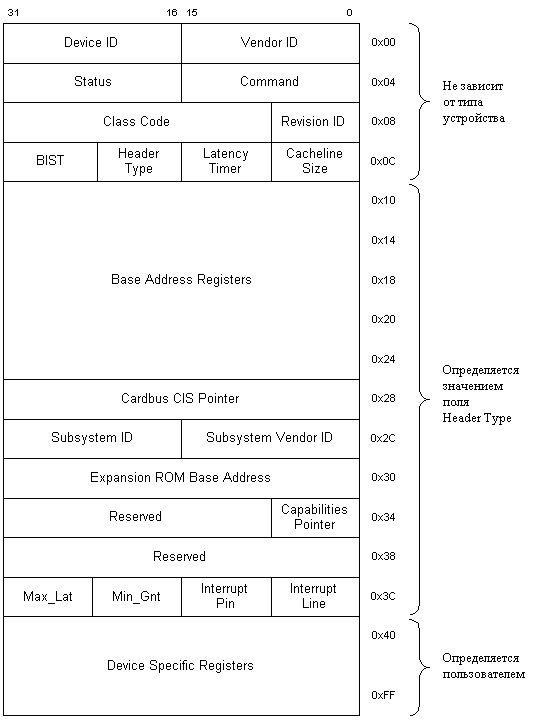
\includegraphics[scale=0.88]{res/pic01}
\caption{Конфигурационное адресное пространство}
\end{figure}

Поля Vendor ID, Device ID и Class Code содержат код фирмы-изготовителя устройства, код устройства и код класса устройства. Классификация устройств и указание кода класса в его конфигурационном пространстве является важной частью спецификации PCI\cite{Cragon}.

Код изготовителя, код устройства и код класса применяются в процессе поиска заданного устройства. Если необходимо найти конкретное устройство, то поиск выполняется по кодам устройства и его изготовителя; если необходимо найти все устройства определенного типа, то поиск выполняется по коду класса устройства. После того как устройство найдено, при помощи регистров базовых адресов можно определить выделенные ему области в адресном пространстве памяти и пространстве ввода-вывода (I/O).

Регистры базовых адресов (Base Address Registers) содержат выделенные устройству области в адресном пространстве и пространстве портов I/O. Бит 0 во всех регистрах базовых адресов определяет, куда будет отображен ресурс – на пространство портов I/O или на адресное пространство. Регистр базового адреса, отображаемый на пространство портов, всегда 32-разрядный, бит 0 установлен в 1. Регистр базового адреса, отображаемый на адресное пространство, может быть 32- и 64-разрядным, бит 0 сброшен в 0.

Использование этих регистров будет продемонстрировано в этой работе далее.